
%(BEGIN_QUESTION)
% Copyright 2011, Tony R. Kuphaldt, released under the Creative Commons Attribution License (v 1.0)
% This means you may do almost anything with this work of mine, so long as you give me proper credit

A control valve is used as a pressure-control device in a geothermal steam system where steam is drawn from several ``production wells'' drilled deep into the earth.  Processes running on this geothermal steam require a constant 600 PSI steam pressure, and so the control system's job is to vent any excess steam as needed to prevent the pressure from exceeding 600 PSI in the ``header'' pipe.  The design priority here is to have a well-regulated (stable) header pressure under normal operating conditions:

$$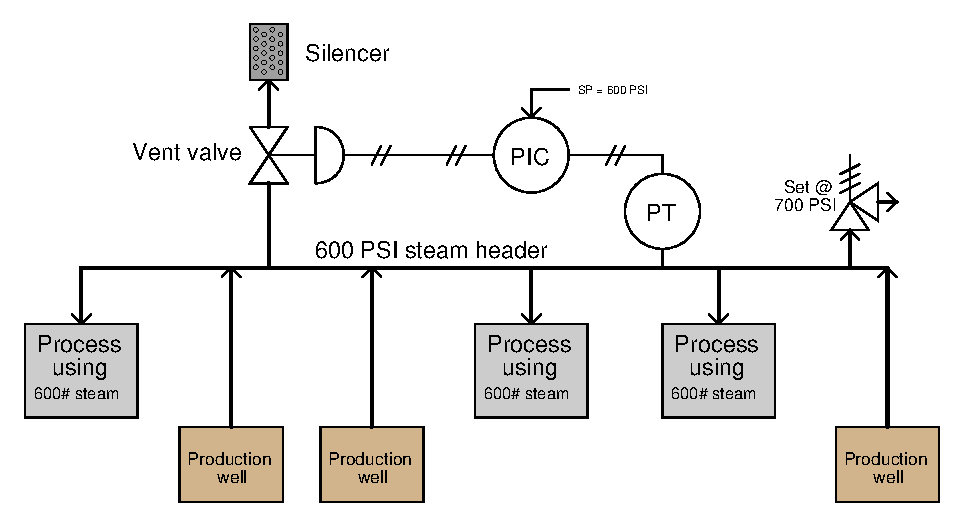
\includegraphics[width=15.5cm]{i04360x01.eps}$$

A fellow instrument technician recommends the use of an {\it equal-percentage} control valve because the silencer (kind of like a big muffler) will drop substantial amounts of pressure dependent on the amount of steam flowing through it.  Another instrument technician disagrees, saying the valve needs to be {\it linear} because the header pressure will always be a steady 600 PSI.  Yet another instrument technician recommends a {\it quick-opening} control valve, because in an emergency situation it is good to have the vent valve open rapidly.  Which technician do you agree with, and why do you think the other two techs are wrong?

\vskip 75pt

Finally, all three technicians recommend that the control valve be specified with {\it anti-cavitation} trim to help it avoid damage from cavitation.  Do you think this is necessary?  Explain why or why not.

\vskip 50pt


\underbar{file i04360}
%(END_QUESTION)





%(BEGIN_ANSWER)

I recommend assigning 2.5 points for making the correct characterization choice ({\bf equal-percent}) and 2.5 points for correct reasoning ({\bf the silencer's significant pressure drop means a flow-dependent $\Delta P$ across the control valve which will ``distort'' the valve's behavior}).

\vskip 10pt

Another 2.5 points awards the answer of {\bf no} with regard to cavitation, and 2.5 more points for the correct reason ({\bf the steam is already a vapor, and will remain a vapor as it travels through the control valve and into the atmosphere, therefore it cannot cavitate}).

%(END_ANSWER)





%(BEGIN_NOTES)

{\bf This question is intended for exams only and not worksheets!}.

%(END_NOTES)


